\documentclass[11pt,openany]{article}

\usepackage{mathtools, commath}
% Packages for formatting
\usepackage[margin=1in]{geometry}
\usepackage{fancyhdr}
\usepackage{enumerate}
\usepackage{graphicx}
\usepackage{kotex}
\usepackage{arydshln} % Include this package
\usepackage{bbding}
\usepackage{amsmath}
\usepackage{amsthm}
\usepackage[dvipsnames,table]{xcolor}
\usepackage{amssymb, amsfonts}
\usepackage{wasysym}
\usepackage{footnote}
\usepackage{tablefootnote}
\usepackage{arydshln} % Include this package

% Fonts
\usepackage[T1]{fontenc}
\usepackage[utf8]{inputenc}
\usepackage{newpxtext,newpxmath}
\usepackage{sectsty}

% Define colors
\definecolor{TealBlue1}{HTML}{0077c2}
\definecolor{TealBlue2}{HTML}{00a5e6}
\definecolor{TealBlue3}{HTML}{b3e0ff}
\definecolor{TealBlue4}{HTML}{00293c}
\definecolor{TealBlue5}{HTML}{e6f7ff}

\definecolor{thmcolor}{RGB}{231, 76, 60}
\definecolor{defcolor}{RGB}{52, 152, 219}
\definecolor{lemcolor}{RGB}{155, 89, 182}
\definecolor{corcolor}{RGB}{46, 204, 113}
\definecolor{procolor}{RGB}{241, 196, 15}

\usepackage{color,soul}
\usepackage{soul}
\newcommand{\mathcolorbox}[2]{\colorbox{#1}{$\displaystyle #2$}}
\usepackage{cancel}
\newcommand\crossout[3][black]{\renewcommand\CancelColor{\color{#1}}\cancelto{#2}{#3}}
\newcommand\ncrossout[2][black]{\renewcommand\CancelColor{\color{#1}}\cancel{#2}}

\usepackage{hyperref}
\usepackage{booktabs}

% Chapter formatting
\definecolor{titleTealBlue}{RGB}{0,53,128}
\usepackage{titlesec}
\titleformat{\section}
{\normalfont\sffamily\Large\bfseries\color{titleTealBlue!100!gray}}{\thesection}{1em}{}
\titleformat{\subsection}
{\normalfont\sffamily\large\bfseries\color{titleTealBlue!50!gray}}{\thesubsection}{1em}{}

%Tcolorbox
\usepackage[most]{tcolorbox}
\usepackage{multirow}
\usepackage{multicol}
\usepackage{blindtext}

\usepackage[linesnumbered,ruled]{algorithm2e}
\usepackage{algpseudocode}
\usepackage{setspace}
\SetKwComment{Comment}{/* }{ */}
\SetKwProg{Fn}{Function}{:}{end}
\SetKw{End}{end}
\SetKw{DownTo}{downto}

% Define a new environment for algorithms without line numbers
\newenvironment{algorithm2}[1][]{
	% Save the current state of the algorithm counter
	\newcounter{tempCounter}
	\setcounter{tempCounter}{\value{algocf}}
	% redefine the algorithm numbering (remove prefix)
	\renewcommand{\thealgocf}{}
	\begin{algorithm}
	}{
	\end{algorithm}
	% Restore the algorithm counter state
	\setcounter{algocf}{\value{tempCounter}}
}

\usepackage{adjustbox}
% Header and footer formatting
\pagestyle{fancy}
\fancyhead{}
\fancyhf{}
\rhead{\textcolor{TealBlue2}{\large\textbf{리만의 복소해석을 토대로 얻는 내 수학적 시야 (2기)}}}%\rule{3cm}{0.4pt}}
\lhead{\textcolor{TealBlue2}{\large\textbf{수학의 즐거움, Enjoying Math}}}
% Define footer
%\newcommand{\footer}[1]{
%\begin{flushright}
%	\vspace{2em}
%	\includegraphics[width=2.5cm]{school_logo.jpg} \\
%	\vspace{1em}
%	\textcolor{TealBlue2}{\small\textbf{#1}}
%\end{flushright}
%}
%\rfoot{\large Department of Information Security, Cryptogrphy and Mathematics, Kookmin Uni.\includegraphics[height=1.5cm]{school_logo.jpg}}
\fancyfoot{}
\fancyfoot[C]{-\thepage-}

\usepackage{animate}
% Load the PDF and grab its total pages into \NumPages:
\newcount\NumPagesA
\pdfximage{../riemann-tikz/secant_line_gif.pdf}% loads the PDF
\NumPagesA=\pdflastximagepages
\usepackage{tcolorbox}
\tcbset{colback=white, arc=5pt}

\definecolor{axiomcolor}{HTML}{a88bfa}
\definecolor{defcolor}{RGB}{52, 152, 219}
\definecolor{procolor}{RGB}{241, 196, 15}
\definecolor{thmcolor}{RGB}{231, 76, 60}
\definecolor{lemcolor}{RGB}{155, 89, 182}
\definecolor{corcolor}{RGB}{46, 204, 113}
\definecolor{execolor}{RGB}{90, 128, 127}

% Define a new command for the custom tcolorbox
\newcommand{\axiombox}[2][]{%
	\begin{tcolorbox}[colframe=axiomcolor, title={\color{white}\bfseries #1}]
		#2
	\end{tcolorbox}
}

\newcommand{\defbox}[2][]{%
	\begin{tcolorbox}[colframe=defcolor, title={\color{white}\bfseries #1}]
		#2
	\end{tcolorbox}
}

\newcommand{\probox}[2][]{%
	\begin{tcolorbox}[colframe=procolor, title={\color{white}\bfseries #1}]
		#2
	\end{tcolorbox}
}

\newcommand{\thmbox}[2][]{%
	\begin{tcolorbox}[colframe=thmcolor, title={\color{white}\bfseries #1}]
		#2
	\end{tcolorbox}
}

\newcommand{\lembox}[2][]{%
	\begin{tcolorbox}[colframe=lemcolor, title={\color{white}\bfseries #1}]
		#2
	\end{tcolorbox}
}
\usepackage{amsthm}

% Define custom theorem styles
\newtheoremstyle{dotless} % Name of the style
{3pt} % Space above
{3pt} % Space below
{\itshape} % Body font
{} % Indent amount
{\bfseries} % Theorem head font
{} % Punctuation after theorem head
{2.5mm} % Space after theorem head
{} % Theorem head spec

\newtheoremstyle{definitionstyle} % Name of the style
{3pt} % Space above
{3pt} % Space below
{} % Body font
{} % Indent amount
{\bfseries} % Theorem head font
{.} % Punctuation after theorem head
{2.5mm} % Space after theorem head
{} % Theorem head spec

% Applying custom styles
%\theoremstyle{dotless}
\newtheorem{theorem}{Theorem} % Theorem environment with section-wise numbering
\newtheorem*{theorem*}{Theorem} % Theorem environment with section-wise numbering
\newtheorem*{lemma*}{Lemma} % Theorem environment with section-wise numbering
\newtheorem*{proposition*}{Proposition} % Theorem environment with section-wise numbering
\newtheorem*{corollary*}{Corollary} % Theorem environment with section-wise numbering
\newtheorem{proposition}[theorem]{Proposition} % Theorem environment with section-wise numbering
\newtheorem{lemma}[theorem]{Lemma} % Lemma shares the counter with theorem
\newtheorem{corollary}[theorem]{Corollary} % Corollary shares the counter with theorem

\theoremstyle{definitionstyle}
\newtheorem*{observation}{\textcolor{magenta}{Observation}}
\newtheorem*{illustration}{\textcolor{teal}{Illustration}}
\newtheorem*{torus}{{\color{red}T}{\color{orange}o}{\color{green!75!black}r}{\color{cyan}u}{\color{violet}s}}
\newtheorem{definition}{Definition} % Definition shares the counter with theorem
\newtheorem{example}{Example} % Example shares the counter with theorem
\newtheorem{exercise}{{Exercise}} % Example shares the counter with theorem
\newtheorem{remark}{Remark} % Remark shares the counter with theorem
\newtheorem*{note}{Note}
\newtheorem*{notation}{Notation}

\newtheorem*{axiom*}{Axiom}
\newtheorem*{definition*}{Definition} % Definition shares the counter with theorem
\newtheorem*{example*}{Example} % Example shares the counter with theorem
\newtheorem*{exercise*}{\textcolor{teal}{Exercise}} % Example shares the counter with theorem
\newtheorem*{remark*}{Remark} % Remark shares the counter with theorem


\usepackage{tikz}
\usepackage{tikz-cd}
\usetikzlibrary{shadows}
\usetikzlibrary{shapes.geometric, arrows.meta, positioning}
\input{riemann-complex-commands}
\renewcommand{\vec}[1]{\mathbf{#1}}
\renewcommand{\emph}[1]{\textbf{#1}}
\renewcommand{\d}{\mathrm{d}} % For the exterior derivative 'd'
\newcommand{\pderiv}[2]{\frac{\partial #1}{\partial #2}}
\newcommand{\spderiv}[3]{\frac{\partial^2 #1}{\partial #2\partial #3}}
\newcommand{\vect}[1]{\begin{bmatrix} #1 \end{bmatrix}}

\newcommand{\circulationsquare}[1]{
	\draw[thick, gray] #1 rectangle ++(1,1);
	\begin{scope}[decoration={markings, mark=at position 0.5 with {\arrow{>}}}]
		\draw[postaction={decorate}, blue] #1 -- ++(1,0);
		\draw[postaction={decorate}, blue] ++(1,0) -- ++(0,1);
		\draw[postaction={decorate}, blue] ++(0,1) -- ++(-1,0);
		\draw[postaction={decorate}, blue] ++(-1,0) -- cycle;
	\end{scope}
}

\usepackage{esvect}
\usepackage{physics}

\setstretch{1.25}

\begin{document}
\pagenumbering{arabic}
\begin{center}
%	\huge\textbf{Riemann; Complex Analysis}\\
	\huge\textbf{From Vector Calculus to Differential Forms}\\
%	\Large - HW1 -\\
	\vspace{0.5em}
	\large{Ji, Yong-hyeon}\\
%	\large{\ttfamily \url{https://github.com/Hacker-Code-J}}\\
	\vspace{0.5em}
	\normalsize{\today}\\
\end{center} 
%\[\boxed{
%\underbrace{f}_{\Omega^0}
%\;\xrightarrow{d}\;
%\underbrace{df}_{\Omega^1}
%\;\longleftrightarrow\;
%\underbrace{\nabla f}_{\substack{\text{gradient}\\\text{vector field}}}
%\quad
%\longrightarrow
%\quad
%\underbrace{\mathbf F}_{(\Omega^0)^m}
%\;\xrightarrow{d}\;
%\underbrace{d\mathbf F}_{\Omega^1\otimes\R^m}
%\;\longleftrightarrow\;
%\underbrace{D\mathbf F}_{\substack{\text{Jacobian}\\\text{matrix}}}}
%\]
\noindent 
We cover the following topics in this note.
\begin{itemize}
	\item Vector calculus (conservative fields, irrotational field)
	\item Differential forms (exact forms, closed forms)
\end{itemize}
%In this note, we build a bridge between the familiar concepts of vector calculus (conservative fields, curl) and the language of differential forms (exact forms, closed forms)
%\hrule\vspace{12pt}
\begin{center}
	\begin{tabular*}{\textwidth}{@{\extracolsep{\fill}} l c l}
		\hline
		\textbf{Vector Calculus (in $\R^2$ or $\R^3$)} & & \textbf{Differential Forms} \\
		\hline
		Vector Field $\vec F$ & $\iff$ & 1-form $\omega$ \\
		Conservative Vector Field ($\vec F = \nabla f$) & $\iff$ & Exact 1-form ($\omega = \d f$) \\
		Irrotational Vector Field ($\nabla \times \vec F = \mathbf{0}$) & $\iff$ & Closed 1-form ($\d\omega = 0$) \\
		\hline
	\end{tabular*}
\end{center}

\vspace{1em}

\begin{framed}
	\noindent\textbf{The Fundamental Implication:}
	\begin{itemize}
		\item \textbf{Conservative $\implies$ Irrotational},\; i.e.,\; \textbf{Exact $\implies$ Closed}\\ (This is always true.)
		\item \textbf{Irrotational $\implies$ Conservative},\; i.e,\; \textbf{Closed $\implies$ Exact}\\ (This is only true on ``nice'' domains, e.g., simply connected ones.)
	\end{itemize}
\end{framed}


\tableofcontents
\newpage

\section{Conservative and Exact}
\subsection*{Why do we think of the ``Conservative Field (or Gradient Field)''?}
A vector field $\vec F$ is \textbf{conservative} if it is the \textbf{gradient}\footnote{Gradient is a measure of change in a scalar field} of some scalar potential function $f$: \[
\vec F = \nabla f=\begin{cases}
	\left\langle\frac{\partial f}{\partial x}, \frac{\partial f}{\partial y} \right\rangle &\text{ if}\; f:U(\subseteq\R^2)\to\R\\
	\left\langle\frac{\partial f}{\partial x}, \frac{\partial f}{\partial y}, \frac{\partial f}{\partial z}\right\rangle &\text{ if}\; f:U(\subseteq\R^3)\to\R\\
	\left\langle\frac{\partial f}{\partial x_1}, \frac{\partial f}{\partial x_2},\dots, \frac{\partial f}{\partial x_n}\right\rangle &\text{ if}\; f:U(\subseteq\R^n)\to\R
\end{cases}.
\] If $\vec F$ is conservative, line integrals only depend on the endpoints: \[
\int_{\gamma}\vec F\cdot \d\vec r= \int_{\gamma}\nabla f\cdot \d\vec r=f(\textrm{end}) - f(\textrm{start}),
\] which turns \textcolor{red}{hard line integrals} into \textcolor{blue}{simple evaluations}. Furthermore every closed loop (start = end) has integral $0$.

Equivalently (on a nice domain) every line integral of $\vec F$ is path-independent: \[
\int_{\gamma_1}\vec F\cdot \d\vec r = \int_{\gamma_2}\vec F\cdot \d\vec r.
\] whenever $\gamma_1$ and $\gamma_2$ have the same endpoints.

\subsection*{From Gradients to Curl}
Given a vector field $\vec F$, we wish to determine whether $\vec F$ is conservative (i.e., $\vec F=\nabla f$ for some scalar field $f$). Trying to guess the potential function $f$ is hard.

We already know that if a field $\vec{F}$ is conservative, it must be the gradient of some potential function $f$:
\[
\vec{F} = \langle P(x,y), Q(x,y) \rangle = \nabla f = \left\langle \pderiv{f}{x}, \pderiv{f}{y} \right\rangle\tag*{\text{(in 2D)}}
\] What happens if we differentiate $P(x,y) = \pderiv{f}{x}$ with respect to $y$ and $Q(x,y) = \pderiv{f}{y}$ with respect to $x$? \[
\pderiv{P}{y} = \pderiv{}{y}\left(\pderiv{f}{x}\right) = \frac{\partial^2 f}{\partial y \partial x},\quad\quad\pderiv{Q}{x} = \pderiv{}{x}\left(\pderiv{f}{y}\right) = \frac{\partial^2 f}{\partial x \partial y}.
\]
\begin{theorem}[Equality of mixed partials; Clairaut's Theorem]
If the partial derivatives $\spderiv{f}{y}{x}$ and $\spderiv{f}{x}{y}$ exist and are continuous at a point $(a, b)$, then $\spderiv{f}{y}{x}(a,b)=\spderiv{f}{x}{y}(a,b)$, i.e., second order partial derivatives commute if $f$ is $C^2$.
\end{theorem}

\newpage\noindent
If a vector field $\vec{F} = \langle P(x,y), Q(x,y) \rangle$ is a gradient, it \textbf{must} satisfy the condition \[
\pderiv{Q}{x} = \pderiv{P}{y}.
\]
The quantity $\frac{\partial Q}{\partial x}-\frac{\partial P}{\partial y}$ represents the curl of $\vec F=\langle P,Q\rangle$ and encodes its local rotational behavior. Hence the condition $\frac{\partial Q}{\partial x}=\frac{\partial P}{\partial y}$ (i.e., $\frac{\partial Q}{\partial x}-\frac{\partial P}{\partial y}=0$) means that the field is \textbf{irrotational} (has \textbf{zero curl}).

\medskip

\begin{remark}
Consider a small rectangle centered at \((x_0,y_0)\) with side lengths \(\Delta x,\Delta y\). 
\begin{figure}[h!]
	\centering
	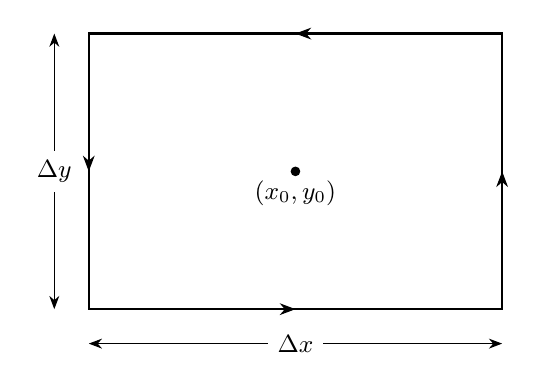
\begin{tikzpicture}[scale=1.75, font=\small, >=Stealth]
		% Draw rectangle and center point
		\draw[thick] (-1.5,-1) rectangle (1.5,1);
		\fill (0,0) circle (1pt) node[below] {$(x_0, y_0)$};
		% Add arrows for CCW circulation path
		\draw[-{Stealth[length=2mm]}] (-1.5, -1) -- (0, -1);
		\draw[-{Stealth[length=2mm]}] (1.5, -1) -- (1.5, 0);
		\draw[-{Stealth[length=2mm]}] (1.5, 1) -- (0, 1);
		\draw[-{Stealth[length=2mm]}] (-1.5, 1) -- (-1.5, 0);
		\draw[<->] (0-1.5, 0-1.25) -- ++(3, 0) node[midway, fill=white] {$\Delta x$};
		\draw[<->] (0-1.75, 0-1) -- ++(0, 2) node[midway, fill=white] {$\Delta y$};
		% Label path segments
%		\node at (0, -1.7) {Bottom: $\int P(x, y_0-\frac{\Delta y}{2}) dx$};
%		\node at (0, 1.45) {Top: $\int P(x, y_0+\frac{\Delta y}{2}) (-dx)$};
%		\node[rotate=90] at (1.95, 0) {Right: $\int Q(x_0+\frac{\Delta x}{2}, y) dy$};
%		\node[rotate=90] at (-2.2, 0) {Left: $\int Q(x_0-\frac{\Delta x}{2}, y) (-dy)$};
		% Illustrate change in P and Q
%		\draw[->, thick, blue] (0, 1) -- (1.2, 1) node[above] {$P_{top}$};
%		\draw[->, thick, blue] (0, -1) -- (0.8, -1) node[below] {$P_{bot}$};
%		\node[red, align=center] at (2.5, 0) {Difference in P\\contributes\\$-P_y \Delta x \Delta y$};
%		\draw[->, thick, green!50!black] (1.5, 0) -- (1.5, 0.8) node[right] {$Q_{right}$};
%		\draw[->, thick, green!50!black] (-1.5, 0) -- (-1.5, 1.0) node[left] {$Q_{left}$};
%		\node[red, align=center] at (-2.5, 0) {Difference in Q\\contributes\\$Q_x \Delta x \Delta y$};
	\end{tikzpicture}
	\caption{Circulation around an infinitesimal rectangle.}
	\label{fig:local_circ}
\end{figure}

\noindent
The total counterclockwise circulation is the sum of the line integrals along the four edges:
\[
\oint_{\partial R}\vec F\cdot \d\vec r
=\int_{\text{bottom}}P\,\d x+\int_{\text{right}}Q\,\d y+\int_{\text{top}}P\,\d x+\int_{\text{left}}Q\,\d y.
\]
We will approximate the value of $P$ or $Q$ along each edge as being constant, equal to its value at the midpoint of that edge. We find this value using a first-order Taylor expansion from the center point $(x_0, y_0)$.

For a simple function of one variable, $f(x)$, if we know its value at a point $a$, then we can estimate its value at a nearly point $a+h$ using the tangent line at $a$: 
\begin{center}
\begin{minipage}{.49\textwidth}
\begin{align*}
	f(a+h)&\approx f(a)+f'(a)\cdot h \quad\text{or}\\
	f(x)&\approx f(a)+f'(a)\cdot (x-a).
\end{align*} 

\end{minipage}
\begin{minipage}{.49\textwidth}
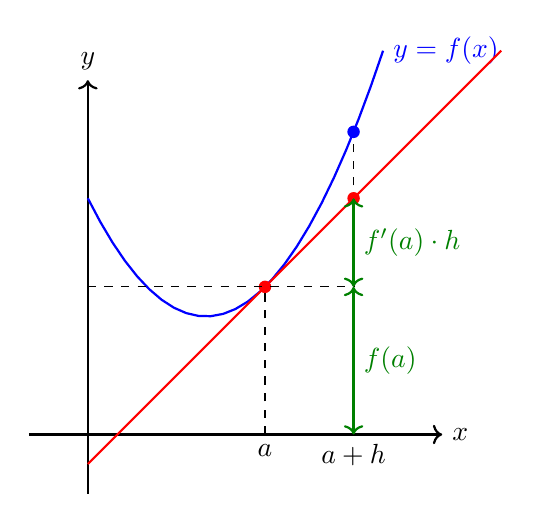
\begin{tikzpicture}[
	scale=1.5,
	declare function={f(\x) = (\x-1)^2 + 1;}
	]
	% Axes
	\draw[->, thick] (-0.5,0) -- (3,0) node[right] {$x$};
	\draw[->, thick] (0,-0.5) -- (0,3) node[above] {$y$};
	% The curve f(x)
	\draw[blue, thick, domain=0:2.5] plot (\x, {f(\x)}) node[right] {$y=f(x)$};
	% Point 'a'
	\def\a{1.5}
	\node[below] at (\a,0) {$a$};
	\draw[dashed] (\a,0) -- (\a, {f(\a)});
	\fill[red] (\a, {f(\a)}) circle (1.5pt);
	% Point 'a+h'
	\def\h{.75}
	\node[below] at (\a+\h,0) {$a+h$};
	\draw[dashed] (\a+\h,0) -- (\a+\h, {f(\a+\h)});
	% Tangent line at 'a'
	% f'(x) = 2(x-1), so f'(a) = 2(a-1)
	\draw[red, thick, domain=0:3.5] plot (\x, {f(\a) + 2*(\a-1)*(\x-\a)});
	% Show f(a)
	\draw[<->, green!50!black, thick] (\a+\h, 0) -- (\a+\h, {f(\a)}) node[midway, right] {$f(a)$};
	% Show the approximation f(a) + f'(a)h
	\pgfmathsetmacro{\approxY}{f(\a) + 2*(\a-1)*\h}
	\fill[red] (\a+\h, \approxY) circle (1.5pt);
%	\draw[red, dashed] (\a+\h, \approxY) -- (\a+\h, 0);
	
	% Show the actual value f(a+h)
	\fill[blue] (\a+\h, {f(\a+\h)}) circle (1.5pt);
%	\node[right, blue] at (\a+\h, {f(\a+\h)}) {Actual value: $f(a+h)$};
%	\node[right, red] at (\a+\h, \approxY) {Approximation: $f(a)+f'(a)h$};
	
	% Label the components of the approximation
	\draw[<->, green!50!black, thick] (\a+\h, {f(\a)}) -- (\a+\h, \approxY) node[midway, right] {$f'(a)\cdot h$};
	\draw[dashed] (0, {f(\a)}) -- (\a+\h, {f(\a)});
\end{tikzpicture}
\end{minipage}
\end{center}
In words, ``New Value $\approx$ Old Value + (Rate of Change) $\times$ (Small Step)''. 

\newpage\noindent
For a function of two variables like $P(x,y)$, the idea is identical, but the ``rate of change'' now has two components (one for each direction), and the ``tangent line'' becomes a ``tangent plane''.
The general first-order Taylor expansion for $P(x,y)$ around a center point $(x_0,y_0)$ is
\[
P(x_0+a, y_0+b) \approx P(x_0, y_0) + \pderiv{P}{x}(x_0, y_0) \cdot a + \pderiv{P}{y}(x_0, y_0) \cdot b
\] Here, $a$ is the small step in the $x$-direction, and $b$ is the small step in the $y$-direction.

\paragraph{1. The Horizontal Paths}
These integrals involve the horizontal component of $P(x,y)$.
\begin{itemize}
	\item \textbf{Bottom Path ($\rightarrow$):} 
	\[ P\left(x, y_0 - \frac{\Delta y}{2}\right) \approx P(x_0,y_0) - \pderiv{P}{y}\frac{\Delta y}{2}\implies
	\int_{\text{bottom}} P\,\d x \approx \left( P(x_0,y_0) - \pderiv{P}{y}\frac{\Delta y}{2} \right) (\Delta x) \]
	\item \textbf{Top Path ($\leftarrow$):}
	\[ P\left(x, y_0 + \frac{\Delta y}{2}\right) \approx P(x_0,y_0) + \pderiv{P}{y}\frac{\Delta y}{2}\implies\int_{\text{top}}P\,\d x \approx -\left( P(x_0,y_0) + \pderiv{P}{y}\frac{\Delta y}{2} \right) (\Delta x) \]
\end{itemize} Here, we are left with only the parts that describe the \textit{change} in $P$ with respect to $y$.
\[
\int_{\text{bottom}} P\,\d x + \int_{\text{top}} P\,\d x \approx \left(-\pderiv{P}{y}\frac{\Delta y}{2}\right)\Delta x - \left(\pderiv{P}{y}\frac{\Delta y}{2}\right)\Delta x = -\pderiv{P}{y}\Delta x\Delta y
\]
\paragraph{2. The Vertical Paths}
These integrals involve the vertical component of $Q(x,y)$.
\begin{itemize}
	\item \textbf{Right Path ( $\uparrow$ ):} 
	\[ Q\left(x_0 + \frac{\Delta x}{2}, y\right) \approx Q(x_0,y_0) + \pderiv{Q}{x}\frac{\Delta x}{2}\implies\int_{\text{right}}Q\,\d y \approx \left( Q(x_0,y_0) + \pderiv{Q}{x}\frac{\Delta x}{2} \right) (\Delta y) \]
	\item \textbf{Left Path ( $\downarrow$ ):} 
	\[ Q\left(x_0 - \frac{\Delta x}{2}, y\right) \approx Q(x_0,y_0) - \pderiv{Q}{x}\frac{\Delta x}{2}\implies\int_{\text{left}}Q\,\d y \approx -\left( Q(x_0,y_0) - \pderiv{Q}{x}\frac{\Delta x}{2} \right) (\Delta y) \]
\end{itemize} Here, we are left with only the parts that describe the \textit{change} in $Q$ with respect to $x$.
\[
\int_{\text{right}}Q\,\d y + \int_{\text{left}}Q\,\d y \approx \left(\pderiv{Q}{x}\frac{\Delta x}{2}\right)\Delta y + \left(\pderiv{Q}{x}\frac{\Delta x}{2}\right)\Delta y = \pderiv{Q}{x}\Delta x\Delta y
\]

Now we sum the results from the horizontal and vertical pairs:
\begin{align*}
	\oint_{\partial R}\vec F\cdot d\vec r &\approx \left(-\pderiv{P}{y}\Delta x\Delta y\right) + \left(\pderiv{Q}{x}\Delta x\Delta y\right) \\
	&= \left(\pderiv{Q}{x} - \pderiv{P}{y}\right)\Delta x\Delta y
\end{align*}
This shows that the total circulation around the tiny loop is approximately the quantity $\left(\pderiv{Q}{x} - \pderiv{P}{y}\right)$ multiplied by the area of the loop ($\Delta A = \Delta x \Delta y$).

To get the property \textit{at the point} $(x_0, y_0)$, we find the circulation \textbf{density}. We divide by the area and take the limit as the rectangle shrinks to zero.
\[
\lim_{\Delta A\to 0}\frac{1}{\Delta A}\oint_{\partial R}\vec F\cdot \d\vec r = \pderiv{Q}{x}(x_0, y_0) - \pderiv{P}{y}(x_0, y_0)
\]
This is why we call the scalar quantity $\pderiv{Q}{x} - \pderiv{P}{y}$ the \textbf{curl}: it is the circulation per unit area at a point, which measures the local rotational tendency of the field.

\end{remark}

\begin{remark}
If \(C=\partial D\) is a positively oriented simple closed curve enclosing a region \(D\),
Green's theorem states \[
%\oint_{C}\vec F\cdot\d\vec r
%=\iint_{D}\Big(\frac{\partial Q}{\partial x}-\frac{\partial P}{\partial y}\Big)\,\d A.
\underbrace{\oint_{C}\vec F\cdot\d\vec r}_{\substack{\textbf{Line Integral}\\ \textbf{(Total Circulation)}}}= \underbrace{\iint_{D}\Big(\frac{\partial Q}{\partial x}-\frac{\partial P}{\partial y}\Big)\,\d A}_{\substack{\textbf{Double Integral}\\ \textbf{(Sum of Local Curls)}}}
\]
%So the total circulation equals the area integral of the local circulation density.
\begin{center}
\begin{tikzpicture}[scale=1.5, >=Stealth]
	% Style for the main curve and region
	\tikzstyle{maincurve}=[thick, blue, postaction={decorate, decoration={markings, mark=at position 0.1 with {\arrow{>}}, mark=at position 0.35 with {\arrow{>}}, mark=at position 0.6 with {\arrow{>}}, mark=at position 0.85 with {\arrow{>}}}}]
	\tikzstyle{mainregion}=[thick, blue, fill=blue!10]
	% 1. Draw the main region D and its boundary C
	\draw[mainregion] plot [smooth cycle, tension=0.7] coordinates {(0,0) (5,1) (6,4) (3,5) (-1,3)};
	\node[blue] at (6.75, 1.5) {\Large $C = \partial D$};
	\draw[maincurve] plot [smooth cycle, tension=0.7] coordinates {(0,0) (5,1) (6,4) (3,5) (-1,3)};
	% Clip the grid to the shape of D
	\begin{scope}
		\clip plot [smooth cycle, tension=.7] coordinates {(0,0) (5,1) (6,4) (3,5) (-1,3)};
		% Draw a faint grid representing dA elements
%		\draw[gray!50, thin, step=1] (-2,-1) grid (8,5);
		\def\step{0.70} % Match the grid step size
		% Loop to draw multiple rectangles
		% x_coord from 0 to 5, y_coord from 1 to 4 (adjust these ranges to cover your desired area)
		\foreach \xcoord in {-2,-1.25, ..., 6} { % Start, step, end for x
			\foreach \ycoord in {0, .75, ..., 4.5} { % Start, step, end for y
				\draw[fill=red] (\xcoord+\step/2,\ycoord+\step/2) circle (2pt);
				% Draw the four edges of each rectangle with the arrow style
				\draw[red, thin, ->] (\xcoord,\ycoord) -- (\xcoord+\step/2,\ycoord);
				\draw[red, thin, -] (\xcoord+\step/2,\ycoord) -- (\xcoord+\step,\ycoord);
				\draw[red, thin, ->] (\xcoord+\step,\ycoord) -- (\xcoord+\step,\ycoord+\step/2);
				\draw[red, thin, -] (\xcoord+\step,\ycoord+\step/2) -- (\xcoord+\step,\ycoord+\step);
				\draw[red, thin, ->] (\xcoord+\step,\ycoord+\step) -- (\xcoord+\step/2,\ycoord+\step);
				\draw[red, thin, -] (\xcoord+\step/2,\ycoord+\step) -- (\xcoord,\ycoord+\step);
				\draw[red, thin, ->] (\xcoord,\ycoord+\step) -- (\xcoord,\ycoord+\step/2);
				\draw[red, thin, ->] (\xcoord,\ycoord+\step/2) -- (\xcoord,\ycoord);
			}
		}
	\end{scope}
\end{tikzpicture}
\end{center}
\end{remark}



\section*{Example 1: Rigid rotation and angular velocity}
Consider the rigid rotation field with angular speed \(\omega\):
\[
\vec F(x,y)=\langle -\omega y,\ \omega x\rangle.
\]
Then
\[
\frac{\partial Q}{\partial x}=\omega,\qquad \frac{\partial P}{\partial y}=-\omega
\quad\Rightarrow\quad
\operatorname{curl}\vec F = Q_x - P_y = 2\omega.
\]
This shows curl equals twice the angular velocity. For a circle of radius \(R\),
parametrize \(r(t)=(R\cos t,R\sin t)\), \(dr=(-R\sin t,R\cos t)\,dt\). Then
\[
\oint \vec F\cdot d\vec r
=\int_0^{2\pi}\omega R^2\,dt
=2\pi\omega R^2.
\]
Meanwhile, \(\iint_{D}(2\omega)\,dA=2\omega \cdot \pi R^2=2\pi\omega R^2\), agreeing with Green's theorem.

\section*{Example 2: Curl-free but not conservative (topology matters)}
On \(\mathbb{R}^2\setminus\{(0,0)\}\), define
\[
\vec F(x,y)=\Big\langle -\frac{y}{x^2+y^2},\ \frac{x}{x^2+y^2}\Big\rangle.
\]
A direct calculation shows \(Q_x-P_y=0\) wherever defined (curl-free). However, the circulation
around the unit circle is
\[
\oint \vec F\cdot d\vec r=2\pi\neq 0.
\]
Hence there is no global potential function; the puncture creates a topological obstruction.
This illustrates that \(\operatorname{curl}\vec F=0\) captures \emph{local} rotation, while global
circulation can persist in domains with holes.

\section*{Summary checklist}
\begin{itemize}
	\item \(Q_x-P_y\) is the infinitesimal (per-area) circulation density.
	\item Green's theorem sums local curl to give total circulation.
	\item Rigid rotation: \(\operatorname{curl}=2\omega\) (twice angular velocity).
	\item Curl \(=0\) can still have nonzero loop integrals if the domain has holes.
\end{itemize}

\newpage
\subsection*{Test 1: Equality of Mixed Partials}
\subsection*{Test 2: Path Independence}
\subsection*{Test 3: Potential Recovery}

%\begin{example}
%Consider the simple vector field $\vec F(x,y) = \langle y, 0 \rangle$.
%
%\begin{center}
%\begin{tikzpicture}
%	\begin{axis}
%		[
%		axis lines = middle,
%		xmin = -3, xmax = 3,
%		ymin = -3, ymax = 3,
%		zmin = 0, zmax = 1,
%		axis equal image,
%		view = {0}{90},
%		]
%		\addplot3
%		[
%		quiver =
%		{
%			u = {y},
%			v = {0},
%		},
%		-stealth,
%		domain = -2:2,
%		domain y = -2:2,
%		red
%		] {0};
%	\end{axis}
%\end{tikzpicture}
%\end{center}
%\end{example}
%
%\begin{tikzpicture}[
%	scale=1.5,
%	font=\Large,
%	% Define styles for different elements
%	vector/.style={-stealth, blue, thick},
%	point/.style={circle, fill, inner sep=1.5pt},
%	label/.style={font=\large},
%	calc/.style={font=\huge, align=left}
%	]
%	% --- Visualization for dP/dy ---
%	\node[label, align=center] at (0, 3) {Horizontal Component ($P=y$)\\changes with $y$};
%	% Draw two points vertically aligned
%	\node[point, label={[label]right: $(x, y)$}] (p1) at (0, 1) {};
%	\node[point, label={[label]right: $(x, y+\Delta y)$}] (p2) at (0, 2) {};
%	% Draw vectors at these points, F=<y,0>
%	\draw[vector] (p1) -- ++(1, 0) node[anchor=west]{$\vv{F}(x,y) = \langle y, 0 \rangle$};
%	\draw[vector] (p2) -- ++(2, 0) node[anchor=west]{$\vv{F}(x,y+\Delta y) = \langle y+\Delta y, 0 \rangle$};
%	% Dashed line to show vertical change
%	\draw[dashed, thick] (p1) -- (p2);
%	\node[calc, green!50!black] at (1.5, 0) {$\pdv{P}{y} = \pdv{}{y}(y) = 1$};
%	
%	% --- Visualization for dQ/dx ---
%	\node[label, align=center] at (5, 3) {Vertical Component ($Q=0$)\\does not change with $x$};
%	% Draw two points horizontally aligned
%	\node[point, label={[label]right: $(x, y)$}] (q1) at (5, 1.5) {};
%	\node[point, label={[label]right: $(x+\Delta x, y)$}] (q2) at (6.5, 1.5) {};
%	% Note that the vertical component is 0 at both points
%	\node[label, gray] at (q1) [below=5pt] {Vertical component $Q=0$};
%	\node[label, gray] at (q2) [below=5pt] {Vertical component $Q=0$};
%	% Dashed line to show horizontal change
%	\draw[dashed, thick] (q1) -- (q2);
%	\node[calc, red] at (6, 0) {$\pdv{Q}{x} = \pdv{}{x}(0) = 0$};
%	
%	% --- Divider Line ---
%	\draw[gray, very thick] (3.5, -1) -- (3.5, 3.5);
%	
%	% --- Final Curl Calculation ---
%	\node[calc, align=center] at (3.5, -2) {
%		Curl = $\underbrace{\pdv{Q}{x}}_{\color{red}0} - \underbrace{\pdv{P}{y}}_{\color{green!50!black}1} = 0 - 1 = -1$
%	};
%\end{tikzpicture}

\newpage
\section{Zero Curl and Closed}
%In $\R^3$, the \textbf{curl} of a vector field $\vec F = \begin{bmatrix}
%	P & Q & R
%\end{bmatrix}^{\top}$ measures its local ``swirl'' or rotation.
%\[\nabla \times \F = \vect{\pderiv{R}{y} - \pderiv{Q}{z} \\[1ex] \pderiv{P}{z} - \pderiv{R}{x} \\[1ex] \pderiv{Q}{x} - \pderiv{P}{y}} \]
\end{document}
